\subsection{Partially implemented concept}\label{conc_implement}

The overall concept presented in chapter \ref{concept} must now be implemented. For this project, an MQTT interface is used. In figure \ref{fig:mqtt_conc_system} one can see a schematic representation of the overall system with an MQTT interface.\\

\begin{figure}[H]
    \centering
    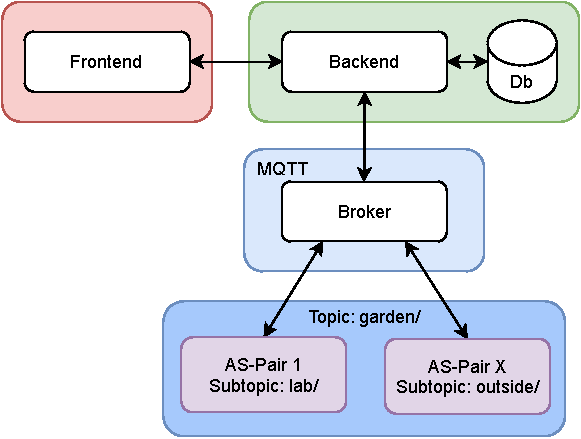
\includegraphics[width=.65\textwidth]{images/4_1/mqtt_concept.pdf}
    \caption{Schematic representation of the system with an MQTT interface}
    \label{fig:mqtt_conc_system}
\end{figure}

For MQTT as an interface, a broker is required for the communication, as described in chapter \ref{theory}.  The broker is located between the backend and AS-Pairs as the central communication system. AS-Pairs that communicate via MQTT can be grouped into different subtopics. In figure \ref{fig:mqtt_conc_system} the AS-Pairs will be grouped under the subtopic \textit{garden/}. Other subtopics can be used for other AS-Pairs subgroups.\\

In this subtopic, different devices can now be differentiated from each other by their own \textit{device topic} like \textit{lab/} or \textit{outside/}. This means that in order to establish communication with eg. AS-Pair 1, one would publish on the topic \textit{garden/lab/}.\\

Thus, AS pairs can be grouped under a special subtask and kept apart eg. by function or place.

\newpage

In figure \ref{fig:hardware_conc_system} one can see the schematic representation of the system which will be used in this project.\\

As already mentioned, this project uses an MQTT interface to communicate with an AS-Pair. The needed broker for an MQTT communication will run on a Raspberry Pi. The frontend, backend and database run on two separate servers.\\

The single AS-Pair, which is addressable under the topic \textit{garden/lab/}, will provide two components, both of which originate from the RWU Board. The potentiometer on channel 0 of the MCP3008 is used as a sensor. The DC motor is used as the actuator, which is controlled via the L239D. An ESP32 forms the middleman between the sensor, the actuator and the MQTT interface to the backend.

\vspace{5mm}
\begin{figure}[H]
    \centering
    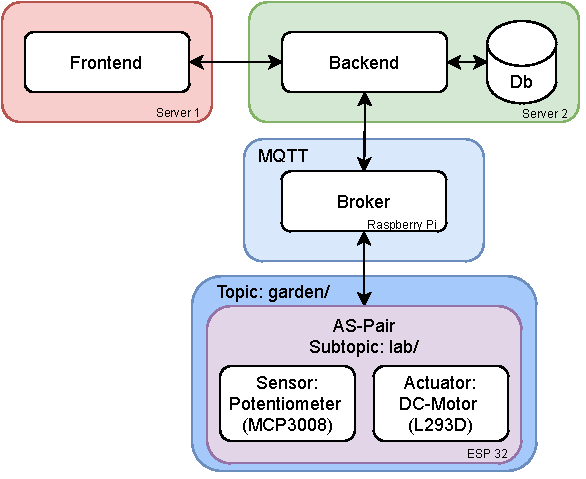
\includegraphics[width=.65\textwidth]{images/4_1/implemented.pdf}
    \caption{Schematic representation of the system used in this project}
    \label{fig:hardware_conc_system}
\end{figure}
